\section{Design Evolution}
\label{sec:evolution}

\subsection{Version 1: a Test Rig}
The first version was not designed for a task. It was a base cut from acrylic sheet, with a
cardboard spacer and a lidar held by bolts, two driven wheels and a caster, and an Intel
RealSense depth camera in a printed holder (\cref{fig:v1}a). I built it while learning
ROS~2 and Gazebo, in order to see the packages that I had run in simulation work with real
sensors. The same robot was modelled in Gazebo Classic, driven from a game controller and
used for lidar mapping.

On the hardware, the output of the lidar and of the depth camera was verified
(\cref{fig:v1}b). Version 1 never carried a payload and had no manipulator.

\begin{figure}[htbp]
  \centering
  \begin{subfigure}[b]{0.56\linewidth}
    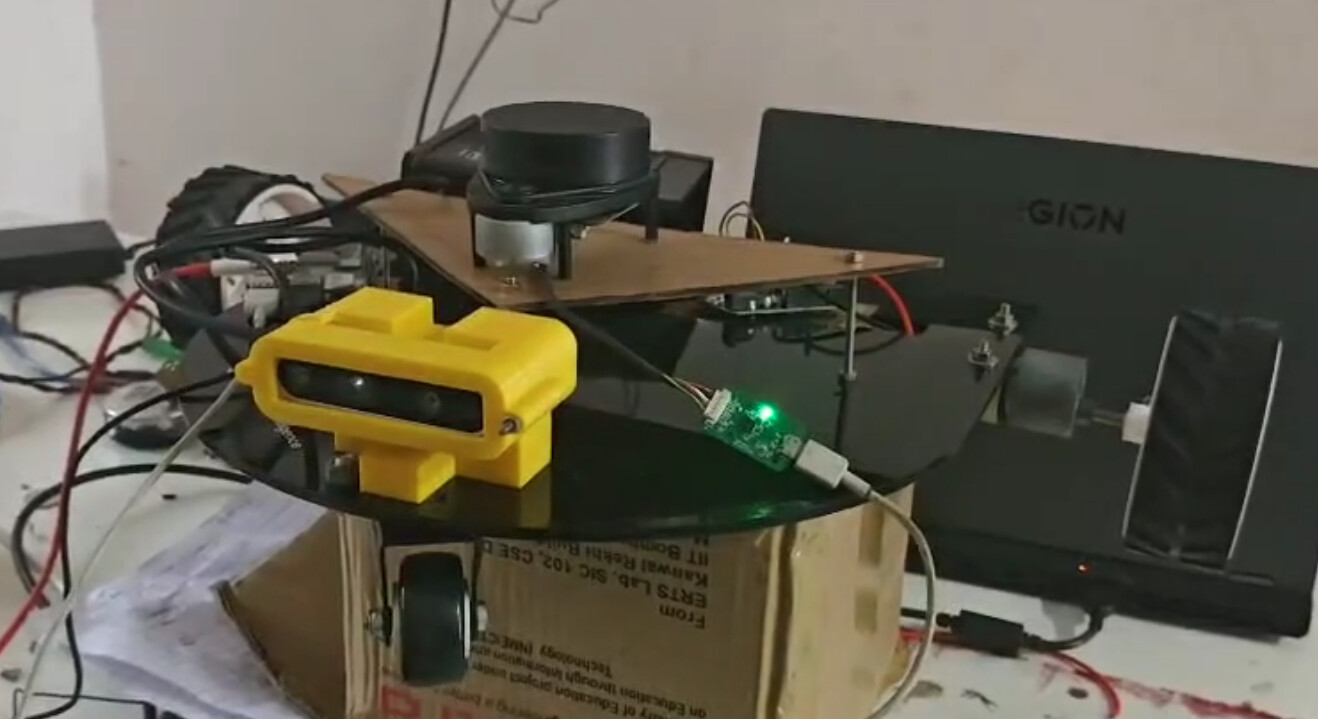
\includegraphics[width=\linewidth]{v1_rig.jpg}
    \caption{The rig with lidar and depth camera}
  \end{subfigure}\hfill
  \begin{subfigure}[b]{0.36\linewidth}
    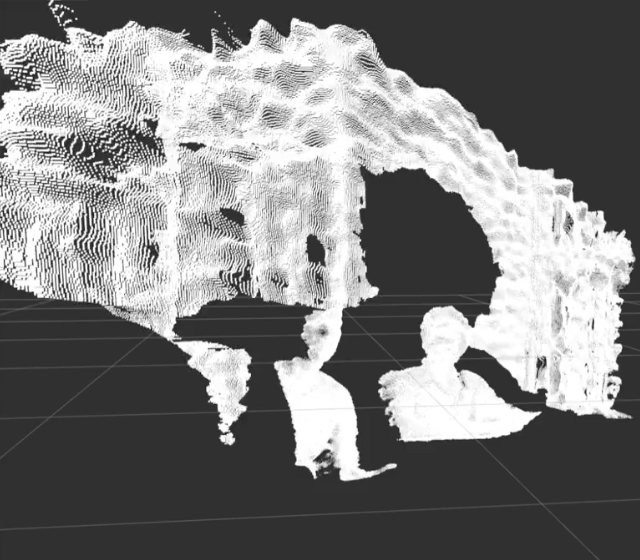
\includegraphics[width=\linewidth]{v1_depth_cloud.png}
    \caption{Depth image of the camera shown as a point cloud}
  \end{subfigure}
  \caption{Version 1, a test rig for sensors and for ROS~2.}
  \label{fig:v1}
\end{figure}

\subsection{Version 2: the Competition Robot}
Version 2 was designed for the task of \cref{sec:introduction}, and from this point the
design was deliberate. The requirements were as follows.
\begin{enumerate}
  \item The centre of mass lies inside the support triangle of the two wheels and the
        caster, so that the robot stands on all three supports.
  \item The robot is small. Motors with high torque do not fit a robot of this size, so N20
        gearmotors drive the wheels.
  \item The gripper holds a cylindrical coin about 40\unit{mm} across and 15\unit{mm} high,
        and it does so wherever the coin first touches it.
  \item The parts are printed, with tolerances that suit the bolts and nuts in use.
\end{enumerate}
The mechanical design and the electronics were completed in fifteen days. In that time the
chassis was printed in more than four iterations, each testing a different tolerance, and the
complete robot went through four iterations. The experience of Version 1 made this pace
possible.

\Cref{fig:v2-line} shows the robot on a test track for the line-following part of the task.

\begin{figure}[htbp]
  \centering
  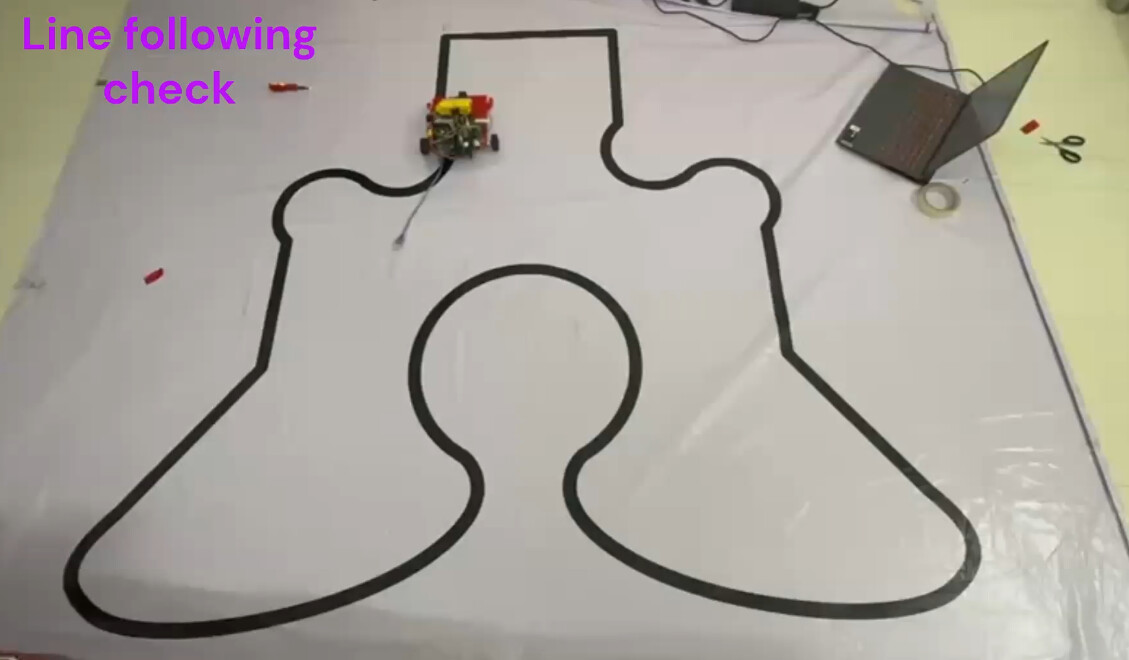
\includegraphics[width=0.62\linewidth]{v2_line_following.jpg}
  \caption{Version 2 following a line on a test track.}
  \label{fig:v2-line}
\end{figure}

\subsection{From the Hardware to the Simulation}
The simulation reported here was written after the competition, from the CAD model of
Version 2. It serves two purposes. It is a place in which the whole mission can be developed
and repeated without the hardware, and it is a check on the design: quantities that were
judged by eye during the fifteen days, such as the load that the wheels carry, can be
read from the model and their consequences calculated. \Cref{sec:mass} does this.
